% mnras_template.tex
%
% LaTeX template for creating an MNRAS paper
%
% v3.0 released 14 May 2015
% (version numbers match those of mnras.cls)
%
% Copyright (C) Royal Astronomical Society 2015
% Authors:
% Keith T. Smith (Royal Astronomical Society)

% Change log
%
% v3.0 May 2015
%    Renamed to match the new package name
%    Version number matches mnras.cls
%    A few minor tweaks to wording
% v1.0 September 2013
%    Beta testing only - never publicly released
%    First version: a simple (ish) template for creating an MNRAS paper

%%%%%%%%%%%%%%%%%%%%%%%%%%%%%%%%%%%%%%%%%%%%%%%%%%
% Basic setup. Most papers should leave these options alone.
\documentclass[a4paper,fleqn,usenatbib]{mnras}

% MNRAS is set in Times font. If you don't have this installed (most LaTeX
% installations will be fine) or prefer the old Computer Modern fonts, comment
% out the following line
\usepackage{newtxtext, newtxmath}
% Depending on your LaTeX fonts installation, you might get better results with one of these:
%\usepackage{mathptmx}
%\usepackage{txfonts}

% Use vector fonts, so it zooms properly in on-screen viewing software
% Don't change these lines unless you know what you are doing
\usepackage[T1]{fontenc}
\usepackage{ae,aecompl}


%%%%% AUTHORS - PLACE YOUR OWN PACKAGES HERE %%%%%

% Only include extra packages if you really need them. Common packages are:
\usepackage{graphicx}	% Including figure files
\usepackage{amsmath}	% Advanced maths commands
\usepackage{amssymb}	% Extra maths symbols

%%%%%%%%%%%%%%%%%%%%%%%%%%%%%%%%%%%%%%%%%%%%%%%%%%

%%%%% AUTHORS - PLACE YOUR OWN COMMANDS HERE %%%%%

% Please keep new commands to a minimum, and use \newcommand not \def to avoid
% overwriting existing commands. Example:
%\newcommand{\pcm}{\,cm$^{-2}$}	% per cm-squared
\newcommand{\fl}[1]{{\color{magenta}FL: #1}}

%%%%%%%%%%%%%%%%%%%%%%%%%%%%%%%%%%%%%%%%%%%%%%%%%%

%%%%%%%%%%%%%%%%%%% TITLE PAGE %%%%%%%%%%%%%%%%%%%

% Title of the paper, and the short title which is used in the headers.
% Keep the title short and informative.
\title[Generative model on graphs]{Deep Generative Model on Graphs for the Empirical Modelling of Intrinsic Alignments}

% The list of authors, and the short list which is used in the headers.
% If you need two or more lines of authors, add an extra line using \newauthor
\author[F. Lanusse et al.]{
Fran\c{c}ois Lanusse,$^{1,2,3,4,5}$\thanks{E-mail: francois.lanusse@gmail.com}
Rachel Mandelbaum,$^{5}$
Siamak Ravanbakhsh,$^{6}$
Ananth Tenneti,$^{5}$
\newauthor
Duncan Campbell,$^{5}$
Tiziana DiMatteo,$^{5}$
Barnabas Poczos$^{6}$
\\
% List of institutions
$^{1}$Berkeley Center for Cosmological Physics, University of California Berkeley, Berkeley, CA, USA\\
$^{2}$Statistics Department, University of California Berkeley, Berkeley, CA, USA\\
$^{3}$Lawrence Berkeley National Laboratory, Berkeley, CA, USA\\
$^{4}$Berkeley Institute for Data Science, University of California Berkeley, Berkeley, CA, USA\\
$^{5}$McWilliams Center for Cosmology, Department of Physics, Carnegie Mellon University, Pittsburgh, PA 15213, USA\\
$^{6}$School of Computer Science, Carnegie Mellon University, Pittsburgh, PA 15213, USA
}

% These dates will be filled out by the publisher
\date{Accepted XXX. Received YYY; in original form ZZZ}

% Enter the current year, for the copyright statements etc.
\pubyear{2018}

% Don't change these lines
\begin{document}
\label{firstpage}
\pagerange{\pageref{firstpage}--\pageref{lastpage}}
\maketitle

% Abstract of the paper
\begin{abstract}
In order to study, and prepare for, potential systematics, upcoming wide-field cosmological surveys require large simulations of the
Universe with realistic galaxy populations. In particular, the tendency of galaxies to naturally align with each other, an effect called 
intrinsic alignments (IA), can be a major source of systematics in the science analysis. As the details of galaxy formation and evolution relevant
to IA cannot be simulated in practice on such volumes, we propose as an  alternative a Deep Generative Model capable of sampling 
the 3D orientations of a population of galaxies as to recover the correct alignments. In our approach, we model the cosmic 
web as a graph, and galaxy orientations as a signal on that graph. The generative model is then based on a Generative 
Adversarial Network architecture and uses specifically designed Graph-Convolutional Networks sensitive to the relative
3D positions of the vertices.
\end{abstract}

% Select between one and six entries from the list of approved keywords.
% Don't make up new ones.
\begin{keywords}
keyword1 -- keyword2 -- keyword3
\end{keywords}

%%%%%%%%%%%%%%%%%%%%%%%%%%%%%%%%%%%%%%%%%%%%%%%%%%

%%%%%%%%%%%%%%%%% BODY OF PAPER %%%%%%%%%%%%%%%%%%

\section{Introduction}

\begin{itemize}
	\item Context
	\item Hydro simulations
	\item Efforts to model IA (for instance Joachimi2012)

\end{itemize}

Upcoming wide-sky cosmological surveys such as LSST or Euclid will aim at answering fundamental questions on the 
nature of Dark Energy, in particular through a precise measurement of cosmic shear, i.e. the minute deformation of distant
galaxy images by the gravitational influence of massive structures along the line of sight. One major astrophysical contaminant
that arises when trying to measure this signal comes from the tendency of galaxies to naturally align with each other, an effect 
called  intrinsic alignments which can mimic cosmic shear, and therefore bias the cosmological analysis. High resolution
hydrodynamical simulations, which can simulate the formation and evolution of individual galaxies, are valuable tools 
to study these alignments, but remain limited to small cosmological volumes due to their computational costs. In this work,
we develop a deep generative model of three-dimensional galaxy orientations which can be trained on hydrodynamical
simulations and then used to sample realistic alignments in much larger N-body simulations at very little cost.

Our approach is to model the cosmic web as a graph, which is a natural data structure to capture the correlations of galaxy properties
amongst neighbours \cite{Coutinho2016}. Given this structure, we adapt a Graph-Convolutional Network \cite{Defferrard2016} to be sensitive
to the 3D relative positions between vertices, a key ingredient to make the model aware of the  Euclidean geometry of the problem beyond the graph connectivity. Using these layers, we subsequently implement a deep Generative Adversarial Network (GAN,  \cite{Goodfellow2014}) for signals on graphs.


\section{Modelling challenges}

	\subsection{Modelling}

	\subsection{Simulations}


\section{Deep Learning Background}

\subsection{Graph Convolutional Networks}

\subsubsection{Spectral graph convolutions}

\fl{Rework this section, maybe some details can be dropped in view of the recent Healpix graph CNN paper}

In this work, we are considering undirected and connected graphs, which can be defined as  $\mathcal{G} = (\mathcal{V} , \mathcal{E}, \mathbf{W})$, where $\mathcal{V}$ is the set of graphs vertices, with $\left\vert \mathcal{V} \right\vert = n$ the number of vertices,  $\mathcal{E}$ is the set of graph edges and $\mathbf{W} \in \mathbb{R}^{n \times  n}$ is the weighted adjacency matrix.

The normalized combinatorial graph  Laplacian is defined at $\mathbf{L} = \mathbf{I} - \mathbf{D}^{-1/2} \mathbf{W} \mathbf{D}^{-1/2}$. Note that this operator is positive semi-definite and therefore  admit an eigenvalue decomposition defined as:
\begin{equation}
	\mathbf{L} = \mathbf{U} \mathbf{\Lambda} \mathbf{U}^t
\end{equation}
where $\mathbf{U}$ is a unitary matrix and $\mathbf{\Lambda} = diag([\lambda_0, \lambda_1, \cdots, \lambda_n])$ are the eigenvalues  of the operator. By analogy with a traditional Euclidean Laplacian, this transform is called a graph Fourier transform, the columns of $\mathbf{U}$ are called graph Fourier modes  and $\mathbf{\Lambda}$ is the diagonal matrix of graph Fourier frequencies. For a given signal $f \in \mathbb{R}^n$, the graph Fourier transform of $x$ is then defined as $\hat{x} = \mathbf{U}^t x$. 

Given this  harmonic transform, it becomes possible to define spectral filtering on graphs by defining a convolution product on graphs as a multiplication in Fourier space:
\begin{equation}
	f  \star g = \mathbf{U} \left( ( \mathbf{U}^t f) \odot  ( \mathbf{U}^t g ) \right) = \mathbf{U} \left(  \hat{f} \odot \hat{g} \right)
\end{equation}
where $\odot$ is the Hadamard product.

While this expression allows for convolution operations  on graphs, it is a costly operation as it first requires a decomposition of the  graph Laplacian as well as dense matrix vector multiplications. 

As an efficient solution to a  full spectral graph  convolution, \cite{Defferrard2016} proposed to use a parametric polynomial filters $g_\theta$, of the form:
\begin{equation}
	g_\theta(\mathbf{L}) = \sum_{k=0}^{K-1} \theta_k \mathbf{L}^k
\end{equation}
Defining a filter in  terms of a polynomial function of the graph Laplacian as the advantage that the filter takes the same simple expression in Fourier space: 
\begin{equation}
	g_\theta(\mathbf{L}) =  \sum_{k=0}^{K-1} \theta_k (\mathbf{U} \mathbf{\Lambda}  \mathbf{U}^t)^k  = \sum_{k=0}^{K-1} \theta_k \mathbf{U} \mathbf{\Lambda}^k \mathbf{U}^t =  \mathbf{U}  g_\theta(\mathbf{\Lambda)} \mathbf{U}^t 
\end{equation}
A graph convolution with such a parametric filter can be defined as $g_\theta \star f = g_\theta(\mathbf{L}) f = \mathbf{U} $.

For a function $f$ the chebychev decomposition of $f$ is given by 
\begin{equation}
	f(x) = \sum\limits_{k=0}^{\infty} b_{k} T_k(x)
\end{equation}
where $T_k$ is the  chebyshev polynomial of order $k$.

An efficient implementation of these graph convolutions usually used in Graph Signal Processing is the Chebyshev approximation. Chebyshev polynomials form an orthogonal basis of $L^2([-1,1], dy/\sqrt{1 - y^2})$ and can be computed recursively as $T_k(x) = 2x T_{k-1}(x) - T_{k-2}(x)$ with $T_0 =1$, $T_1 = x$.  

One can therefore define a spectral graph convolution in terms of a finite order Chebyshev polynomial:
\begin{equation}
	g_\theta = \sum_{k=0}^K \theta_k T_k(\Lambda)
\end{equation}

\fl{Detail how this works exactly}

\subsubsection{Directional convolution kernels}

The GCN introduced above uses the same isotropic convolution kernels for the entire graph. However, given the  nature of our signal, we expect the 3D positions of neighbouring galaxies to be relevant to their alignments, for instance we know that within a halo, satellites tend to align towards the central galaxy. We therefore want to design graph convolutions that have some sensitivity to 3D orientations. 

Based on the dynamic convolution kernels introduced in \cite{dynamic}, we propose the following direction-dependent graph convolution layer:
\begin{equation}
	y_i=  \mathbf{b} +  \sum\limits_{m=1}^{M} \frac{1}{|\mathcal{N}_i|} \sum_{j \in \mathcal{N}_i} q_m(x_i, x_j) \mathbf{W}_m x_j 
\end{equation}
where the  $q_m(x_i, x_j)$ are normalized so that $\sum_{m=1}^{M} q_m{x_i, x_j} = 1$ and defined as:

\begin{equation}
		q_m(x_i, x_j) = \exp(- d_m \cdot (x_j - x_i))
\end{equation}

\fl{Finish explanation of directional convolutions, and mention link to structured gcnn}


\subsection{Generative Adversarial Networks}

\begin{itemize}
	\item Explain the concept
	\item Explain the idea behing the Wasserstein metric
	\item Explain  the  Gradient penalty stuff
\end{itemize}


\section{WGCGAN for IA modeling}

In this section we describe the details of the generative model we develop specifically for the modeling of 
intrinsic aligments.




\subsection{Graph construction}


\subsection{Generative model architecture}

\subsection{Training and evaluation}

\section{Results}

\subsection{One-point functions}

	\subsubsection{Stellar mass function}

\begin{figure}
    \centering
    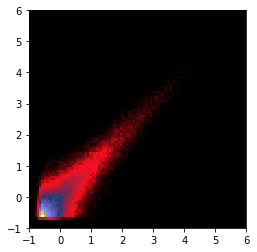
\includegraphics[width=0.5\columnwidth]{Figures/mStar_pred}
    \caption{Predicted stellar mass vs true stellar mass (arbitrary units for now)}
    \label{fig:my_label}
\end{figure}

	\subsection{Galaxy shapes}

\begin{figure}
    \centering
    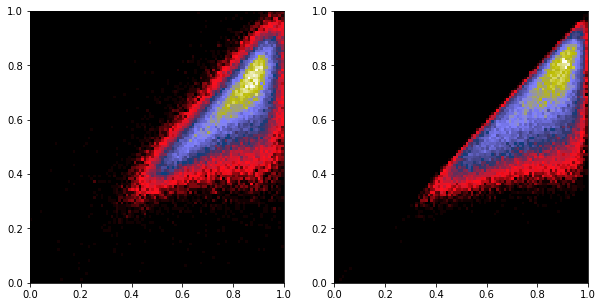
\includegraphics[width=\columnwidth]{Figures/qs_plot}
    \caption{Mock shape parameters (left), MB2 distribution (right)}
    \label{fig:my_label}
\end{figure}

\subsection{Two-point functions}

	\subsection{3D shape correlation functions}

    \begin{figure}
        \centering
        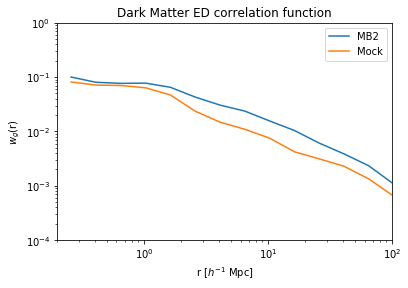
\includegraphics[width=\columnwidth]{Figures/ED_DM}
        \caption{Recovery of dark matter sub-halo alignments from positions and mass only}
        \label{fig:my_label}
    \end{figure}

	\subsection{Projected correlation functions}

\subsection{Halo orientation}

\fl{We could test our ability to predict host halo shapes and orientation for Duncan's model}

\section{Conclusions}


The last numbered section should briefly summarize what has been done, and describe
the final conclusions which the authors draw from their work.

\section*{Acknowledgements}

%The Acknowledgements section is not numbered. Here you can thank helpful
%colleagues, acknowledge funding agencies, telescopes and facilities used etc.
%Try to keep it short.

%%%%%%%%%%%%%%%%%%%%%%%%%%%%%%%%%%%%%%%%%%%%%%%%%%

%%%%%%%%%%%%%%%%%%%% REFERENCES %%%%%%%%%%%%%%%%%%

% The best way to enter references is to use BibTeX:

%\bibliographystyle{mnras}
%\bibliography{example} % if your bibtex file is called example.bib


%%%%%%%%%%%%%%%%%%%%%%%%%%%%%%%%%%%%%%%%%%%%%%%%%%

%%%%%%%%%%%%%%%%% APPENDICES %%%%%%%%%%%%%%%%%%%%%
%
%\appendix
%
%\section{Some extra material}
%

%%%%%%%%%%%%%%%%%%%%%%%%%%%%%%%%%%%%%%%%%%%%%%%%%%


% Don't change these lines
\bsp	% typesetting comment
\label{lastpage}
\end{document}

% End of mnras_template.tex
